\textbf{Ejemplo 9}\\
Elaborar una tabla para amortizar la suma de  100.000 COP en 4 pagos, suponiendo una tasa del 8\% periódica anual vencida:
\begin{itemize}
	\item a. Crecimiento geométrico periódico de 10\% de los flujos
	\item b. Decrecimiento geométrico periódico de 10\% de los flujos
\end{itemize}
	
	%%%%%%%%%%%%%%%%%%% EJERCICIO 9a %%%%%%

%\newpage %USAR SOLO SI EL SOLUCIÓN QUEDA SOLO Y ES NECESARIO BAJARLO A LA SIGUIENTE PAGINA
\textbf{Solución a.}\\
%La tabla ira centrada
\begin{center}
	\renewcommand{\arraystretch}{1.6}% Margenes de las celdas
	%Creación de la cuadricula de 3 columnas
	\begin{longtable}[H]{|c|c|c|}
		%Creamos una linea horizontal
		\hline
		%Definimos el color de la primera fila
		\rowcolor[HTML]{FFB183}
		%%%%% INICIO ASIGNACIÓN FECHA FOCAL %%%%%%%
		%%%%%%%%%% INICIO TITULO
		%Lo que se hace aquí es mezclar las 3 columnas en una sola
		\multicolumn{3}{|c|}{\cellcolor[HTML]{FFB183}\textbf{1. Asignación período focal}}  \\ \hline
		\multicolumn{3}{|c|}{$pf = \textit{0 pav}$}   \\\hline
		%%%%%%%%%% FIN TITULO
		%%%%% INICIO DECLARACIÓN DE VARIABLES %%%%%%%
		%%%%%%%%%% INICIO TITULO
		%Lo que se hace aquí es mezclar las 3 columnas en una sola
		\multicolumn{3}{|c|}{\cellcolor[HTML]{FFB183}\textbf{2. Declaración de variables}}   \\ \hline
		%%%%%%%%%% FIN TITULO
		%%%%%%%%%% INICIO DE MATEMÁTICAS
		%Cada & hace referencia al paso de la siguiente columna
		\multicolumn{2}{|c|}{$\hspace{2 cm}R=  100{.}000 COP \hspace{2 cm}$} & $i=8\% \textit{ pav}$ \\
		\multicolumn{2}{|c|}{$\hspace{2 cm}n=4  \textit{ pav} \hspace{2 cm}$} & $g=10\% \textit{creicente geometrico periódico con } g \neq i$ \\ \hline	
		
		
		%%%%%%%%%% FIN DE MATEMÁTICAS
		%%%%% FIN DECLARACIÓN DE VARIABLES
		
		%%%%% INICIO FLUJO DE CAJA
		\rowcolor[HTML]{FFB183}
		\multicolumn{3}{|c|}{\cellcolor[HTML]{FFB183}\textbf{3. Diagrama de flujo de caja}} \\ \hline
		%Mezclamos 3 columnas y pondremos el dibujo
		%%%%%%%%%%%%% INSERCIÓN DE LA IMAGEN
		%Deberán descargar las imágenes respectivas del drive y pegarlas en la carpeta
		%n_capitulo/img/ejemplos/1/capitulo1ejemplo1.pdf  (el /1/ es el numero del ejemplo)
		\multicolumn{3}{|c|}{ 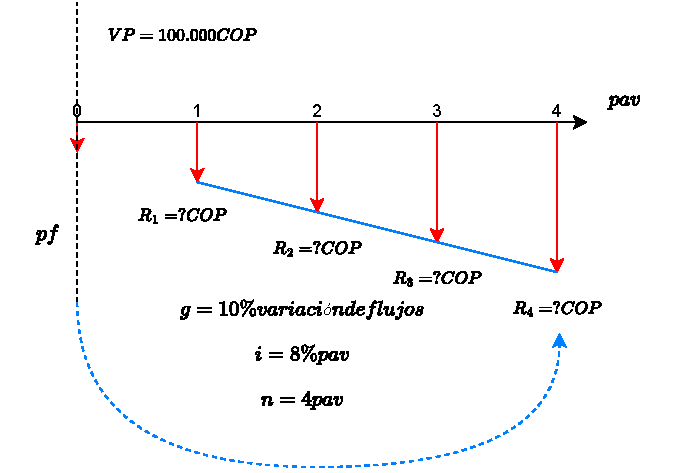
\includegraphics[trim=-5 -5 -5 -5 , scale=0.6]{6_Capitulo/img/ejemplos/9/Capitulo6Ejemplo9a.pdf} }
		\\ \hline
		%%%%%%%%%%%%% FIN INSERCIÓN DE IMAGEN
		%%%%%FIN FLUJO DE CAJA
		
		%%%%% INICIO DECLARACIÓN FORMULAS
		%%%%%%%%%%% INICIO TITULO
		\rowcolor[HTML]{FFB183}
		\multicolumn{3}{|c|}{\cellcolor[HTML]{FFB183}\textbf{4. Declaración de fórmulas}}    \\ \hline
		%%%%%%%%%%% FIN TITULO
		%%%%%%%%%%% INICIO MATEMÁTICAS
		\multicolumn{3}{|c|}{$VP=(\frac{(R)[(1+g)^{n}(1+i)^{-n}-1]}{g-i}) \hspace{0.4 cm} \textit{Valor presente de un gradiente aritmético }$} \\  
		\multicolumn{3}{|c|}{$R_n=(R_1(1+g)^{n-1}) \hspace{0.4 cm} \textit{Valor del flujo de n gradiente geométrico}$} \\ \hline
		
		%%%%%%%%%% FIN MATEMÁTICAS
		%%%%%% INICIO DESARROLLO MATEMÁTICO
		\rowcolor[HTML]{FFB183}
		%%%%%%%%%%INICIO TITULO
		\multicolumn{3}{|c|}{\cellcolor[HTML]{FFB183}\textbf{5. Desarrollo matemático}}       \\ \hline
		%%%%%%%%%% FIN TITULO
		%%%%%%%%%% INICIO MATEMÁTICAS
		\multicolumn{3}{|c|}{$100{.}000COP=(\frac{(R_1)[(1+0.1)^{4}(1+0.08)^{-4}-1]}{0.1-0.08})$} \\
		\multicolumn{3}{|c|}{$R_1=  26{.}261.47 COP$}\\ 
		\multicolumn{3}{|c|}{$R_2=  26{.}261.47(1+0.1) COP=   28{.}887.61COP$}\\
		\multicolumn{3}{|c|}{$R_3=  26{.}261.47(1+0.1)^2 COP=   31{.}776.38COP$}\\
		\multicolumn{3}{|c|}{$R_4=  26{.}261.47(1+0.1)^3 COP=   34{.}954.01COP$}\\ \hline
		%%%%%%%%%% FIN MATEMÁTICAS
		%%%%%% FIN DESARROLLO MATEMÁTICO
		%%%%%% INICIO RESPUESTA
		\rowcolor[HTML]{FFB183}
		%%%%%%%%%%INICIO TITULO
		\multicolumn{3}{|c|}{\cellcolor[HTML]{FFB183}\textbf{6. Respuesta}}   \\ \hline
		%%%%%%%%%% FIN TITULO
		%%%%%%%%%% INICIO RESPUESTA MATEMÁTICA
		\multicolumn{3}{|c|}{$R_1=  26{.}261COP$}\\ 
		\multicolumn{3}{|c|}{$R_2=  28{.}888 COP$}\\
		\multicolumn{3}{|c|}{$R_3=  31{.}776 COP$}\\
		\multicolumn{3}{|c|}{$R_4=  34{.}954 COP$}\\ \hline
		%%%%%%%%%% FIN MATEMÁTICAS
		%%%%%% FIN RESPUESTA
	\end{longtable}
	%Se crean dos lineas en blanco para que no quede el siguiente texto tan pegado
	%\newline \newline %USARLO SI CREES QUE ES NECESARIO
\end{center}

%%%%%%%%%%%%%%%%%%%%%%%%%%FIN EJERCICIO 9a %%%%%%%%%%%%%%%%%%%%%%%%%%%
	      \begin{spacing}{1.1}
	      	\begin{center}
	      		\begin{tabular}{|p{1cm}|p{2cm}|p{2.1cm}|p{2cm}|p{3cm}|}
	      			\hline
	      			\rowcolor{white!50}
	      			\textbf{n\ } & \textbf{Saldo Deuda COP} & \textbf{Intereses  COP} & \textbf{Pago COP} & \textbf{Amortización COP } \\ \hline
	      			
	      			0            &   100.000         &      -       &   -    &        -      \\ \hline
	      			1            &   81.739             &   8.000           &   26.261       &   18.261            \\ \hline
	      			2            &   59.390             &   6539,13              &   28.888       &   22.348,88              \\ \hline
	      			3            &   32.365.21            &   4751,2             &   31.776      &   27.024,79              \\ \hline
	      			4            &   0            &   2589,22            &   34.954       &   32.365,21              \\ \hline
	      		\end{tabular}
	      	\end{center}
	      \end{spacing}

	%%%%%%%%%%%%%%%%%%% EJERCICIO 9b %%%%%%

%\newpage %USAR SOLO SI EL SOLUCIÓN QUEDA SOLO Y ES NECESARIO BAJARLO A LA SIGUIENTE PAGINA
\textbf{Solución b.}\\
%La tabla ira centrada
\begin{center}
	\renewcommand{\arraystretch}{1.6}% Margenes de las celdas
	%Creación de la cuadricula de 3 columnas
	\begin{longtable}[H]{|c|c|c|}
		%Creamos una linea horizontal
		\hline
		%Definimos el color de la primera fila
		\rowcolor[HTML]{FFB183}
		%%%%% INICIO ASIGNACIÓN FECHA FOCAL %%%%%%%
		%%%%%%%%%% INICIO TITULO
		%Lo que se hace aquí es mezclar las 3 columnas en una sola
		\multicolumn{3}{|c|}{\cellcolor[HTML]{FFB183}\textbf{1. Asignación período focal}}  \\ \hline
		\multicolumn{3}{|c|}{$pf = \textit{0 pav}$}   \\\hline
		%%%%%%%%%% FIN TITULO
		%%%%% INICIO DECLARACIÓN DE VARIABLES %%%%%%%
		%%%%%%%%%% INICIO TITULO
		%Lo que se hace aquí es mezclar las 3 columnas en una sola
		\multicolumn{3}{|c|}{\cellcolor[HTML]{FFB183}\textbf{2. Declaración de variables}}   \\ \hline
		%%%%%%%%%% FIN TITULO
		%%%%%%%%%% INICIO DE MATEMÁTICAS
		%Cada & hace referencia al paso de la siguiente columna
		\multicolumn{2}{|c|}{$\hspace{2 cm}VP= 100{.}000 COP \hspace{2 cm}$} & $i=8\% \textit{ pav}$ \\
		\multicolumn{2}{|c|}{$\hspace{2 cm}n=4  \textit{ pav} \hspace{2 cm}$} & $g=-10\% \textit{decreicente con } g \neq i$ \\ \hline	
		
		%%%%%%%%%% FIN DE MATEMÁTICAS
		%%%%% FIN DECLARACIÓN DE VARIABLES
		
		%%%%% INICIO FLUJO DE CAJA
		\rowcolor[HTML]{FFB183}
		\multicolumn{3}{|c|}{\cellcolor[HTML]{FFB183}\textbf{3. Diagrama de flujo de caja}} \\ \hline
		%Mezclamos 3 columnas y pondremos el dibujo
		%%%%%%%%%%%%% INSERCIÓN DE LA IMAGEN
		%Deberán descargar las imágenes respectivas del drive y pegarlas en la carpeta
		%n_capitulo/img/ejemplos/1/capitulo1ejemplo1.pdf  (el /1/ es el numero del ejemplo)
		\multicolumn{3}{|c|}{ 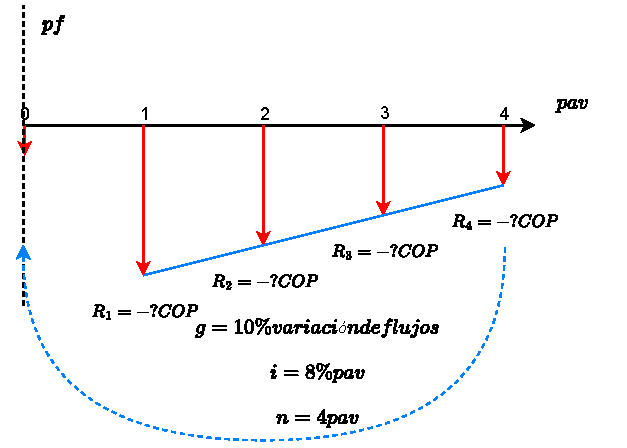
\includegraphics[trim=-5 -5 -5 -5 , scale=0.6]{6_Capitulo/img/ejemplos/9/Capitulo6Ejemplo9b.pdf} }
		\\ \hline
		%%%%%%%%%%%%% FIN INSERCIÓN DE IMAGEN
		%%%%%FIN FLUJO DE CAJA
		
		%%%%% INICIO DECLARACIÓN FORMULAS
		%%%%%%%%%%% INICIO TITULO
		\rowcolor[HTML]{FFB183}
		\multicolumn{3}{|c|}{\cellcolor[HTML]{FFB183}\textbf{4. Declaración de fórmulas}}    \\ \hline
		%%%%%%%%%%% FIN TITULO
		%%%%%%%%%%% INICIO MATEMÁTICAS
		\multicolumn{3}{|c|}{$VP=(\frac{(R)[(1+g)^{n}(1+i)^{-n}-1]}{g-i}) \hspace{0.4 cm} \textit{Valor presente de un gradiente aritmético }$} \\  
		\multicolumn{3}{|c|}{$R_n=(R_1(1+g)^{n-1}) \hspace{0.4 cm} \textit{Valor del flujo de n gradiente geométrico}$} \\ \hline
		
		%%%%%%%%%% FIN MATEMÁTICAS
		%%%%%% INICIO DESARROLLO MATEMÁTICO
		\rowcolor[HTML]{FFB183}
		%%%%%%%%%%INICIO TITULO
		\multicolumn{3}{|c|}{\cellcolor[HTML]{FFB183}\textbf{5. Desarrollo matemático}}       \\ \hline
		%%%%%%%%%% FIN TITULO
		%%%%%%%%%% INICIO MATEMÁTICAS
		\multicolumn{3}{|c|}{$  100{.}000COP=(\frac{(R_1)[(1-0.1)^{4}(1+0.08)^{-4}-1]}{-0.1-0.08})$} \\
		\multicolumn{3}{|c|}{$R_1=  34{.}766 COP$}\\ 
		\multicolumn{3}{|c|}{$R_2=  34{.}766.02COP(1-0.1)  =   31{.}289.42COP$}\\
		\multicolumn{3}{|c|}{$R_3=  34{.}766.02COP(1-0.1)^2 =   28{.}160.48COP$}\\
		\multicolumn{3}{|c|}{$R_4=  34{.}766.02COP(1-0.1)^3 =   25{.}344.43COP$}\\ \hline
		%%%%%%%%%% FIN MATEMÁTICAS
		%%%%%% FIN DESARROLLO MATEMÁTICO
		%%%%%% INICIO RESPUESTA
		\rowcolor[HTML]{FFB183}
		%%%%%%%%%%INICIO TITULO
		\multicolumn{3}{|c|}{\cellcolor[HTML]{FFB183}\textbf{6. Respuesta}}   \\ \hline
		%%%%%%%%%% FIN TITULO
		%%%%%%%%%% INICIO RESPUESTA MATEMÁTICA
		\multicolumn{3}{|c|}{$R_1=  34{.}766COP$}\\ 
		\multicolumn{3}{|c|}{$R_2=  31{.}289COP$}\\
		\multicolumn{3}{|c|}{$R_3=  28{.}160COP$}\\
		\multicolumn{3}{|c|}{$R_4=  25{.}344COP$}\\ \hline
		%%%%%%%%%% FIN MATEMÁTICAS
		%%%%%% FIN RESPUESTA
	\end{longtable}
	%Se crean dos lineas en blanco para que no quede el siguiente texto tan pegado
	%\newline \newline %USARLO SI CREES QUE ES NECESARIO
\end{center}

%%%%%%%%%%%%%%%%%%%%%%%%%%FIN EJERCICIO 9b %%%%%%%%%%%%%%%%%%%%%%%%%%%
	      
	      \begin{spacing}{1.1}
		      \begin{center}
			      \begin{tabular}{|p{1cm}|p{2cm}|p{2.1cm}|p{2cm}|p{2.5cm}|}
				      \hline
				      \rowcolor{white!50}
				      \textbf{n\ } & \textbf{Saldo Deuda COP} & \textbf{Intereses COP } & \textbf{Pago COP } & \textbf{Amortización COP} \\ \hline
				      
				      0            &   100.000         & -    & -  & -    \\ \hline
				      1            &   73.234           &   8.000          &   34.766      &   26.766             \\ \hline
				      2            &   47.803,72           &   5858,72             &   31.289      &   25.430,28             \\ \hline
				      3            &   23.468,01           &   3824,29             &   28.160      &   24.335,7            \\ \hline
				      4            &   0               &   1877,44             &   25.344,73      &   23.468,01             \\ \hline
			      \end{tabular}
		      \end{center}
	      \end{spacing}
